\documentclass[conference]{IEEEtran}

% -------------------- Packages --------------------
\usepackage{cite}
\usepackage{amsmath,amssymb}
\usepackage{graphicx}
\usepackage{booktabs}
\usepackage{tikz}
\usepackage{xcolor}
\usepackage{pgfplots}
\pgfplotsset{compat=newest}
\usepackage[hidelinks]{hyperref}

% -------------------- Document --------------------
\begin{document}

\title{Historical Case Study on Ti Silicide (TiSi\textsubscript{2})\\
Reliability Issues in Legacy CMOS Driver ICs}

\author{
\IEEEauthorblockN{Shinichi Samizo}
\IEEEauthorblockA{Independent Semiconductor Researcher\\
Project Design Hub, Samizo-AITL\\
\textit{Email:} \href{mailto:shin3t72@gmail.com}{shin3t72@gmail.com}\quad
\textit{GitHub:} \href{https://github.com/Samizo-AITL}{Samizo-AITL}}
}

\maketitle

% -------------------- Abstract --------------------
\begin{abstract}
This paper analyzes a historical failure case at the 0.25\,\textmu m CMOS node related to Ti silicide (TiSi\textsubscript{2}) phase-transition instability. 
For active-matrix TFT (aTFT) LCD driver ICs that required mixed 3.3~V logic and $\sim$30~V devices, manufacturers selected the 0.25\,\textmu m node because its LOCOS isolation safely supported high-voltage (HV) co-integration; the 0.18\,\textmu m STI-based node, although denser and yield-stable, posed edge-thinning risks for $\sim$30~V devices. 
Under this context, incomplete C49$\rightarrow$C54 transformation with boron absorption created localized high-resistance spots, directly reducing 1~Mbit SRAM yield.
The study highlights how process optimization and empirical feedback cycles were indispensable when isolation technology and device requirements constrained node selection.
\end{abstract}

% -------------------- Introduction --------------------
\section{Introduction}
In the late 1990s, LCD drivers for monochrome passive panels were commonly fabricated in 0.35\,\textmu m processes supporting 3.3~V logic and 40~V HV devices.
With the shift to color aTFT panels in the early 2000s, driver ICs required higher-performance logic, embedded large SRAM macros, and continued HV device integration around 30~V.

Although the 0.18\,\textmu m CMOS process was already in mass production with small die size and stable yield, it relied on Shallow Trench Isolation (STI), where edge thinning introduced a reliability risk for $\sim$30~V devices.
By contrast, the 0.25\,\textmu m process used Local Oxidation of Silicon (LOCOS), which had a proven track record for HV isolation.
Therefore, manufacturers adopted the 0.25\,\textmu m LOCOS-based process for 3.3~V + 30~V LCD driver ICs, accepting area disadvantages to guarantee HV compatibility.

% -------------------- Full-width Table --------------------
\begin{table*}[t]
  \centering
  \caption{Comparison of 0.25\,\textmu m (LOCOS) and 0.18\,\textmu m (STI) nodes for LCD driver ICs}
  \label{tab:node-comparison}
  \begin{tabular}{lcc}
    \toprule
    & \textbf{0.25\,\textmu m (LOCOS)} & \textbf{0.18\,\textmu m (STI)} \\
    \midrule
    Isolation method      & LOCOS (thick field oxide)             & STI (trench isolation; edge thinning at isolation corners) \\
    HV device support     & Proven $\sim$30~V integration          & New HV platform needed; 30~V reliability risk to be re-validated \\
    Chip size / density   & Larger die; lower density              & Smaller die; higher density \\
    Yield stability       & Moderate (silicide/C49 risk dominant)  & Generally stable baseline process \\
    Adoption rationale    & Safe HV co-integration with aTFT logic & Not adopted for HV driver products at that time \\
    \bottomrule
  \end{tabular}
\end{table*}

% -------------------- Technical Background --------------------
\section{Technical Background}
\subsection{Isolation Choice for HV Devices}
\begin{itemize}
  \item \textbf{0.25\,\textmu m LOCOS}: mature, thick field oxide; well-established margins for $\sim$30~V device isolation.
  \item \textbf{0.18\,\textmu m STI}: shallow trench isolation; better density, but isolation-corner thinning required a new HV device development and qualification flow.
\end{itemize}

\subsection{Ti Silicide Issues}
TiSi\textsubscript{2} was adopted for low resistivity but requires a C49$\rightarrow$C54 phase transformation during RTA.
If the transformation is incomplete, residual C49 grains remain as high-resistance regions.
Boron absorption from halo implants into Ti/TiSi\textsubscript{2} aggravated local resistivity variation.
These effects were largely latent at smaller memory macros (e.g., 500~kbit), but became visible when the array scaled to 1~Mbit.

% -------------------- Failure Analysis --------------------
\section{Failure Analysis}
\subsection{Observation: 1 Mbit SRAM}
In mass production, random single-bit failures appeared in the 1~Mbit SRAM macro.
Because redundancy was not implemented in the embedded macro, even one defective bit caused device rejection.

\subsection{Root Cause}
Failure localization indicated that:
\begin{itemize}
  \item Halo boron was partially absorbed into Ti during silicide formation.
  \item The local B uptake inhibited C54 formation, leaving high-resistance C49 regions.
  \item These high-resistance spots manifested as random SRAM cell failures.
\end{itemize}

\subsection{Review Limitation}
Earlier products integrating 500~kbit SRAM macros had not shown this issue.
Based on those precedents, the team assumed that scaling to 1~Mbit would be acceptable.
Consequently, the failure mode was not identified during the initial development review stage.

% -------------------- Yield Model Figure --------------------
\begin{figure}[t]
  \centering
  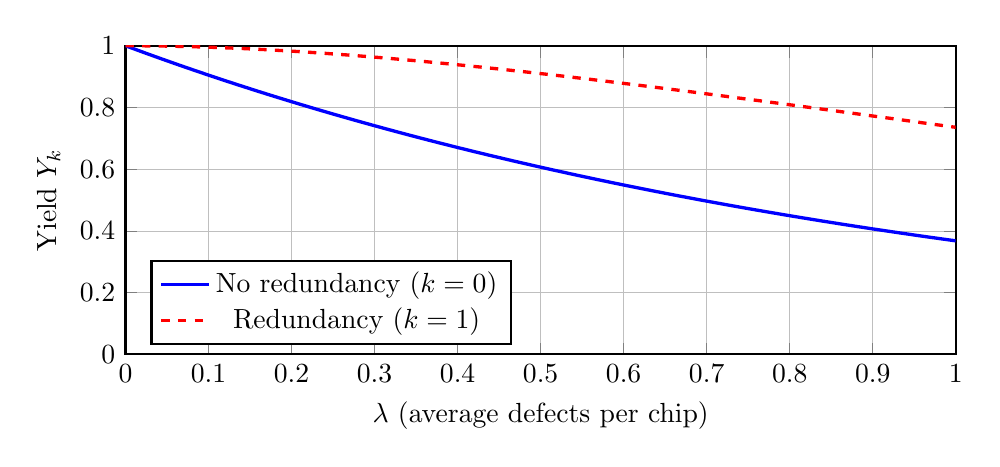
\begin{tikzpicture}
    \begin{axis}[
      width=\linewidth,
      height=5.5cm,
      xlabel={$\lambda$ (average defects per chip)},
      ylabel={Yield $Y_k$},
      xmin=0, xmax=1,
      ymin=0, ymax=1,
      legend pos=south west,
      grid=both,
      major grid style={line width=.2pt,draw=gray!50},
      minor grid style={line width=.1pt,draw=gray!20},
      thick
    ]
      % k = 0  (no redundancy): Y = exp(-λ)
      \addplot[blue, very thick, domain=0:1, samples=200]{exp(-x)};
      \addlegendentry{No redundancy ($k=0$)}
      % k = 1  (one spare): Y = exp(-λ)*(1+λ)
      \addplot[red, dashed, very thick, domain=0:1, samples=200]{exp(-x)*(1+x)};
      \addlegendentry{Redundancy ($k=1$)}
    \end{axis}
  \end{tikzpicture}
  \caption{Illustrative yield sensitivity (Poisson model) with and without redundancy.}
  \label{fig:yield}
\end{figure}

% -------------------- Countermeasures --------------------
\section{Countermeasures}
\subsection{Provisional}
Etch profiles were tuned to slightly undercut sidewalls, increasing separation between halo regions and Ti, which improved yield significantly.

\subsection{Permanent}
RTA conditions were optimized to favor stable C54 formation.
However, this altered device parameters and required re-characterization of process/device models.

% -------------------- Educational Application --------------------
\section{Educational Application}
\subsection{Teaching Tools}
\begin{itemize}
  \item Cause–effect diagrams: process $\rightarrow$ defect $\rightarrow$ yield.
  \item Comparative table: 0.25\,\textmu m (LOCOS) vs.\ 0.18\,\textmu m (STI) for HV devices (Table~\ref{tab:node-comparison}).
  \item Exercises: prioritize process improvement vs.\ introduce redundancy.
\end{itemize}

\subsection{Lessons}
Relying only on 500~kbit SRAM yield data led to an incorrect assumption at 1~Mbit.
Given STI was not yet qualified for 30~V devices at that time, 0.25\,\textmu m LOCOS was the only feasible platform—yet it carried a silicide-instability risk that required explicit mitigation.

% -------------------- Conclusion --------------------
\section{Conclusion}
This case demonstrates how HV compatibility constraints can dominate node selection.
Despite the availability of a denser, yield-stable 0.18\,\textmu m STI process, the need for safe $\sim$30~V integration drove adoption of 0.25\,\textmu m LOCOS.
Yield loss from incomplete TiSi\textsubscript{2} phase transformation (with boron absorption) became critical at the 1~Mbit SRAM scale.
The educational value lies in showing how scaling, isolation technology, and process reliability intersect, and why continuous empirical feedback is essential.

% -------------------- References (single title) --------------------
\section*{References}
\begin{thebibliography}{99}
\bibitem{Sze2007}
S.~M. Sze and K.~K. Ng, \emph{Physics of Semiconductor Devices}, 3rd ed.\ Wiley, 2007.
\bibitem{WolfTauber1986}
S.~Wolf and R.~N. Tauber, \emph{Silicon Processing for the VLSI Era, Vol.~1: Process Technology}.\ Lattice Press, 1986.
\bibitem{Colinge2004}
J.-P. Colinge, \emph{Silicon-on-Insulator Technology: Materials to VLSI}, 3rd ed.\ Springer, 2004.
\bibitem{ITRS2001}
International Technology Roadmap for Semiconductors (ITRS), ``Process Integration, Devices, and Structures,'' 2001.
\bibitem{Takeda1994}
E.~Takeda, C.~Y. Yang, and A.~S. Grove, ``Silicide technology for ULSI applications,'' \emph{IEEE Trans. Electron Devices}, vol.~41, no.~12, pp.~2133--2141, Dec.~1994.
\bibitem{ChangSteckl1996}
J.~P. Chang and A.~J. Steckl, ``Titanium silicide formation and stability in submicron CMOS technology,'' \emph{J. Appl. Phys.}, vol.~79, no.~9, pp.~4536--4364, 1996.
\end{thebibliography}

% -------------------- Author Bio --------------------
\section*{Author Biography}
\textbf{Shinichi Samizo} received the M.S. degree in Electrical and Electronic Engineering from Shinshu University, Japan.
He worked at Seiko Epson Corporation on semiconductor memory and mixed-signal device development, and contributed to inkjet MEMS actuators and PrecisionCore printhead technology.
He is currently an independent semiconductor researcher focusing on process/device education, memory architecture, and AI system integration.\\
\emph{Contact:} \href{mailto:shin3t72@gmail.com}{shin3t72@gmail.com}\quad
\emph{GitHub:} \href{https://github.com/Samizo-AITL}{Samizo-AITL}.

\end{document}
